\documentclass[tikz,border=2pt]{standalone}
\usepackage{amsmath}
\usepackage{pgfplots}
\pgfplotsset{compat=1.18}
\usetikzlibrary{arrows.meta}
\begin{document}
% Definition 2.2 and Property 2.3, Example 2: V = triangle with corners (-7,-8), (-1,4), (2,1); a=(2,1).
% max of 2x1+x2 on V is 5, attained only at (2,1): {2x1+x2=5} supports V; {2x1+x2=4} cuts V (fails (a));
% {2x1+x2=6} keeps V on one side but does not touch it (fails (b)).
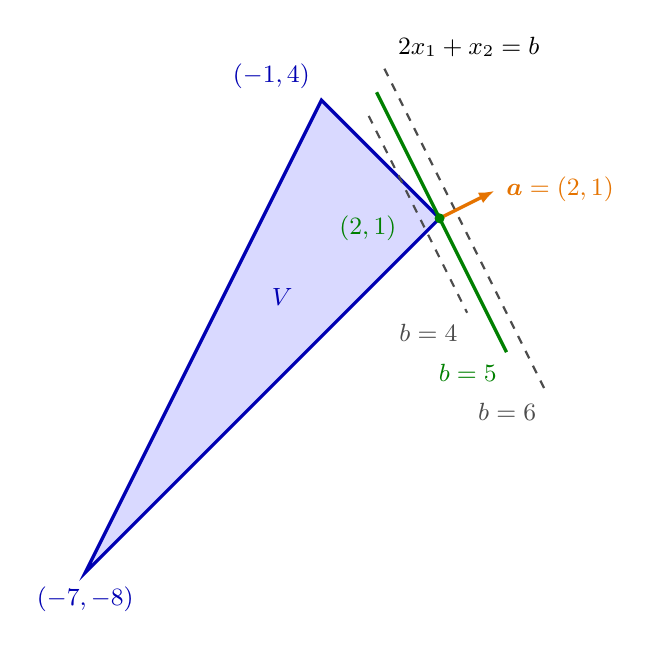
\begin{tikzpicture}[font=\small, >={Latex[length=2mm]}, x=0.5cm, y=0.5cm]
  % V
  \fill[blue!15] (-7,-8) -- (-1,4) -- (2,1) -- cycle;
  \draw[blue!70!black, very thick] (-7,-8) -- (-1,4) -- (2,1) -- cycle;
  \node[blue!70!black] at (-2,-1) {$V$};
  \node[blue!70!black, anchor=north] at (-7,-8.1) {$(-7,-8)$};
  \node[blue!70!black, anchor=south east] at (-1.05,4.05) {$(-1,4)$};
  % level lines 2x1+x2=b
  \draw[gray!60!black, thick, dashed] (0.2,3.6) -- (2.7,-1.4);
  \draw[green!50!black, very thick] (0.4,4.2) -- (3.7,-2.4);
  \draw[gray!60!black, thick, dashed] (0.6,4.8) -- (4.7,-3.4);
  \node[gray!60!black, anchor=north east] at (2.7,-1.45) {$b=4$};
  \node[green!50!black, anchor=north east] at (3.7,-2.45) {$b=5$};
  \node[gray!60!black, anchor=north east] at (4.7,-3.45) {$b=6$};
  \node[anchor=south west] at (0.7,4.85) {$2x_1+x_2=b$};
  % normal a=(2,1)
  \draw[orange!90!black, very thick, ->] (2,1) -- (3.4,1.7);
  \node[orange!90!black, anchor=west] at (3.45,1.75) {$\boldsymbol{a}=(2,1)$};
  % touching point
  \fill[green!50!black] (2,1) circle (1.8pt);
  \node[green!50!black, anchor=east] at (1.15,0.75) {$(2,1)$};
\end{tikzpicture}
\end{document}
